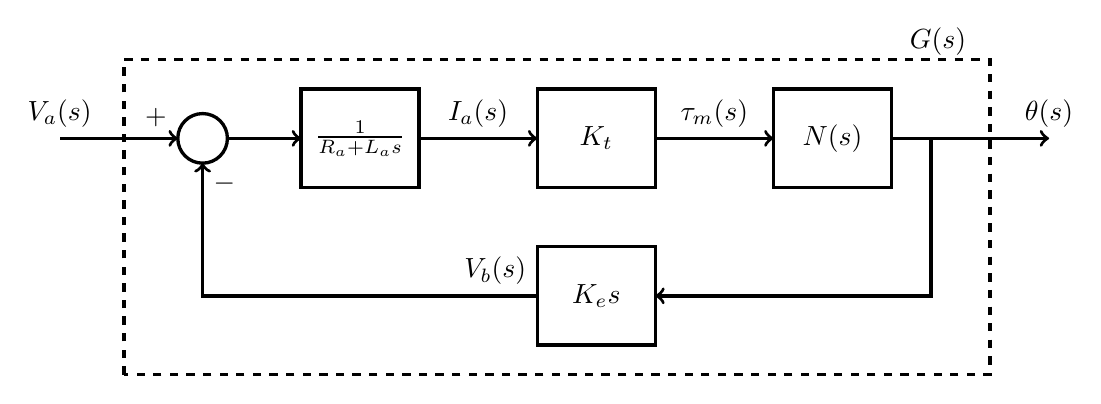
\begin{tikzpicture}[inner sep=0pt,outer sep=0pt,very thick,
sysblock/.style={draw,rectangle,inner sep=2pt,minimum width=1.5cm,minimum height=1.25cm,very thick}]

\draw (0,0) node[draw,circle] (sum) {$\rule{0pt}{18pt}$};
\draw (2,0) node[sysblock] (a) {$\frac{1}{R_{a} + L_{a}s}$};
\draw (5,0) node[sysblock] (b) {$K_{t}$};
\draw (8,0) node[sysblock] (c) {$N(s)$};
\draw (5,-2) node[sysblock] (d) {$K_{e}s$};

\draw[<-] (sum.180) node[above left=4pt] {$+$} -- ++(-1.5,0) node[above=4pt] {$V_{a}(s)$};
\draw[->] (sum.0) -- (a.180);
\draw[->] (a.0) -- node[pos=.5,above=4pt] {$I_{a}(s)$} (b.180);
\draw[->] (b.0) -- node[pos=.5,above=4pt] {$\tau_{m}(s)$} (c.180);
\draw[->] (c.0) -- ++(2,0) node[above=4pt] {$\theta(s)$} node[above left=30pt] {$G(s)$};
\draw[->] (c.0) -- ++(.5,0) |- (d.0);
\draw[->] (d.180) node[above left=4pt] {$V_{b}(s)$} -| (sum.-90) node[below right=4pt] {$-$};

\draw [dashed] (sum) ++(-1,-3) rectangle ++(11,4);

\end{tikzpicture}